\documentclass[conference,a4paper]{IEEEtran}
\usepackage[T1]{fontenc}
\usepackage{amsmath,amssymb}
\usepackage{graphicx}
\usepackage{booktabs}
\usepackage{url}
\usepackage[hidelinks]{hyperref}
\graphicspath{{figures/}}

\begin{document}
\title{DualNet-AL: A Bi-Network Meta-Learning Framework\\for Multi-Class Active Learning}
\author{\IEEEauthorblockN{Himansh Raj, Om Narayan Pandey, and Jaswinder Singh}
\IEEEauthorblockA{School of Computer Science \& Engineering, IILM University, Greater Noida, India\\
\{himansh.raj.cs27, om.pandey.cs27, jaswinder.singh\}@iilm.edu}}
\maketitle

\begin{abstract}
Pool-based active learning reduces annotation cost by letting a model choose which unlabelled images to label, but single-criterion strategies are brittle: uncertainty sampling picks redundant or outlying samples, a single model reinforces its own errors, and at small budgets the model's uncertainty is itself unreliable. We present DualNet-AL, which trains two architecturally different convolutional networks, scores every unlabelled sample with five complementary signals (uncertainty, inter-network disagreement, representativeness, diversity and class balance), fuses them with weights adapted online by a meta-learner, and, in its second version (v2), combines a budget-aware prior that favours typical samples while labels are scarce with cluster-based batch construction. The configuration was chosen on validation data only and evaluated on held-out seeds and the official test splits. Across Fashion-MNIST, SVHN and CIFAR-10 (100$\to$900 labels), DualNet-AL v2 improves the area under the learning curve over random sampling by 2.41, 4.38 and 1.46 percentage points, winning on each of the 3 held-out seeds of every dataset; it is the best of nine methods on SVHN and CIFAR-10 and more than doubles the worst-class recall of random sampling on SVHN (40.5\% vs 16.7\%). Code, per-run logs and a one-command demo are publicly available.
\end{abstract}

\begin{IEEEkeywords}
active learning, deep learning, meta-learning, query by committee, label efficiency, image classification
\end{IEEEkeywords}

\section{Introduction}
Supervised deep networks need many labelled examples, and labelling is the dominant cost in most applied projects.
Active learning (AL) trains on a small labelled set and repeatedly asks an oracle to label the samples the current
model considers most useful~\cite{settles2009}. Classical acquisition functions rank samples by a single criterion:
predictive entropy~\cite{lewis1994}, the margin between the two most likely classes~\cite{scheffer2001},
disagreement within a committee~\cite{seung1992}, or mutual information under model uncertainty
(BALD)~\cite{houlsby2011,gal2017}. Diversity-based methods instead cover the feature space, e.g. the core-set
approach~\cite{sener2018}.

Each criterion fails in a predictable way. Uncertainty-driven batches are redundant and drawn towards outliers; a
single model choosing its own training data reinforces its own mistakes; and at low budgets uncertainty is a poor
guide and typical samples should be preferred~\cite{hacohen2022}. The best criterion therefore depends on the
dataset and on how many labels have been collected.

DualNet-AL addresses these failure modes together. Our contributions are: (i) a bi-network learner whose members
differ in architecture and normalisation, so their disagreement is an informative committee-style signal; (ii) five
rank-normalised acquisition signals fused by a meta-learner that re-weights them every round from measured
validation gain and label-revealed errors; (iii) a selection rule (v2) that adds a budget-aware typicality prior and
one-sample-per-cluster batches; and (iv) a leak-free evaluation of nine strategies under identical networks and
compute, with code and per-run logs released at \url{https://github.com/iamthehimansh/DualNet-AL_Motion}.

\section{Related Work}
\textit{Uncertainty and committees.} Entropy~\cite{lewis1994} and margin~\cite{scheffer2001} sampling are strong,
cheap baselines; query by committee~\cite{seung1992} measures disagreement among several models, and
BALD~\cite{houlsby2011,gal2017} approximates a Bayesian committee with Monte-Carlo dropout. Co-training~\cite{blum1998}
showed the value of two different views of the data, which motivates two architecturally different networks.

\textit{Diversity and batch construction.} Core-set selection~\cite{sener2018} picks a $k$-center cover of the
embedding space; BADGE~\cite{ash2020} combines uncertainty and diversity in gradient space; pre-clustering
\cite{nguyen2004} selects representatives of clusters; learning loss~\cite{yoo2019} trains an auxiliary loss predictor.

\textit{Learned and budget-aware strategies.} Konyushkova et al.~\cite{konyushkova2017} learn an acquisition function
from data and Hsu and Lin~\cite{hsu2015} choose among strategies with a bandit. Hacohen et al.~\cite{hacohen2022} show
that typical samples help at low budgets and uncertain ones at high budgets. DualNet-AL combines a bandit-style
meta-learner over signals with an explicit schedule from typicality to informativeness.

\section{Method}
\subsection{Problem setting}
We start from a labelled set $L$ of 100 random samples and an unlabelled pool $U$. In each of $R=8$
rounds a batch of $B=100$ samples is selected from $U$, labelled by the oracle and moved to $L$, after which
the model is retrained. The goal is maximum test accuracy at every budget.

\subsection{Bi-network learner}
Net~A is a 6-layer $3\times3$ CNN with BatchNorm and max-pooling (289k parameters for RGB
input); Net~B is a wide $5\times5$ CNN with GroupNorm, LeakyReLU, average pooling and an MLP head
(169k parameters). Both are retrained from scratch each round for 300 AdamW steps and their
softmax outputs are averaged. Their concatenated penultimate features form the embedding used for
representativeness, diversity and clustering (Fig.~\ref{fig:arch}).

\begin{figure*}[t]
\centering
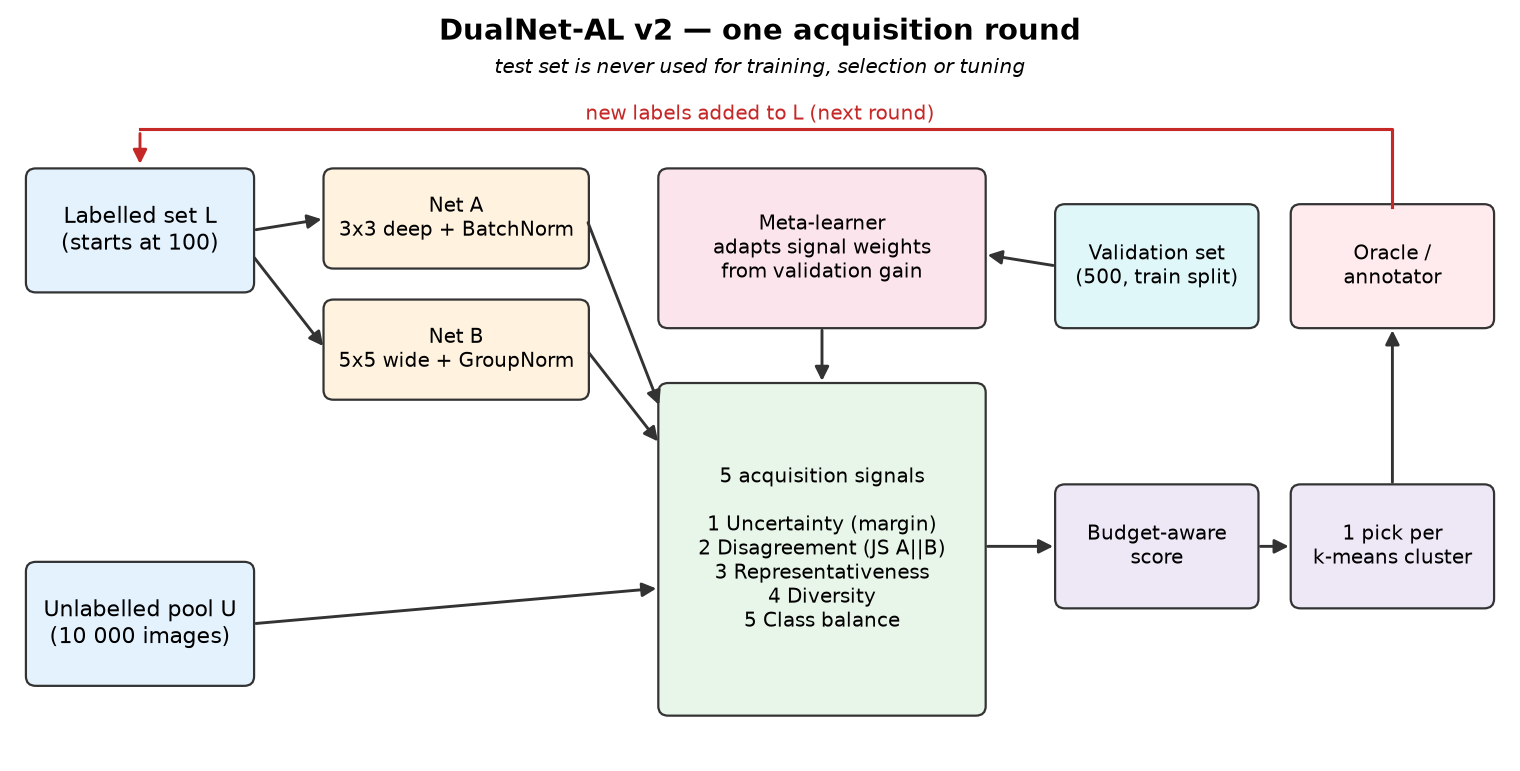
\includegraphics[width=0.86\textwidth]{architecture.png}
\caption{DualNet-AL v2: one acquisition round. The test set is never used for training, selection or tuning.}
\label{fig:arch}
\end{figure*}

\subsection{Acquisition signals}
Each pool sample receives five scores, each mapped to $[0,1]$ by rank-percentile normalisation:
uncertainty $s_1 = 1-(\bar p_{(1)}-\bar p_{(2)})$, the margin of $\bar p=(p_A+p_B)/2$~\cite{scheffer2001};
disagreement $s_2 = 0.7\,\mathrm{JS}(p_A\|p_B)/\log 2 + 0.3\,[\arg\max p_A \neq \arg\max p_B]$ using the
Jensen--Shannon divergence~\cite{lin1991}; representativeness $s_3$, the mean cosine similarity to the 10 nearest pool
neighbours; diversity $s_4$, the distance to the closest labelled sample~\cite{sener2018}; and class balance $s_5$, the
rarity of the predicted class in $L$.

\subsection{Meta-learned weighting}
Signals are fused as $S(x)=\sum_k w_k s_k(x)$ with $w = w_{\min} + (1-5w_{\min})\,\mathrm{softmax}(\theta)$,
$w_{\min}=0.05$, so no signal is switched off. After the batch chosen in round $t$ has been labelled and the networks
retrained,
\begin{equation}
\theta_k \leftarrow \theta_k + \eta\, a\, c_k + \eta_c\, \rho_k ,
\end{equation}
where $a$ is the validation-accuracy gain normalised against a moving baseline (a REINFORCE-style
advantage~\cite{williams1992}), $c_k$ is the batch mean of $s_k$ minus its pool mean, and $\rho_k$ is the correlation
between $s_k$ and the ensemble's errors on the newly labelled batch; $\eta=1.5$, $\eta_c=0.8$.

\subsection{Budget-aware clustered selection (v2)}
Version~1 ranked samples by $S$ and removed near-duplicates. Version~2 scores
\begin{align}
\mathrm{score}(x) &= (1-\lambda_t)\,s_3(x)+\lambda_t\,S(x), \\
\lambda_t &= \lambda_0+(1-\lambda_0)\min(1,\,t/r),
\end{align}
so early rounds favour typical samples~\cite{hacohen2022} and the meta-learned score takes over after $r$ rounds. The
pool embedding is partitioned into $B$ clusters by cosine $k$-means with $k$-means++ seeding~\cite{arthur2007} on the
GPU, and the best-scoring sample of each cluster is selected~\cite{nguyen2004}. The chosen setting is
$\lambda_0=0.5$, $r=4$ with margin uncertainty (Section~\ref{sec:tune}).

\section{Experimental Setup}
\subsection{Datasets and protocol}
We use Fashion-MNIST~\cite{xiao2017}, SVHN~\cite{netzer2011} and CIFAR-10~\cite{krizhevsky2009}. For each dataset and
seed, a 10\,000-image pool and a 500-image validation set are drawn from the official training split and 2\,000 test
images from the official test split; inputs are standardised with pool statistics only. Every strategy starts from
the same 100 random labels for a given seed, adds 100 per round for 8 rounds, and uses the
same networks and training budget; only the selection rule differs. Accuracy is that of the A+B ensemble.

\subsection{Baselines and metrics}
We compare Random, Entropy~\cite{lewis1994}, Margin~\cite{scheffer2001}, BALD with 10 MC-dropout
passes~\cite{gal2017}, Core-Set $k$-center greedy~\cite{sener2018}, QBC over our two networks~\cite{seung1992}, and
DualNet-AL v1 with fixed and with meta-learned weights. The main metric is the area under the accuracy-vs-labels
curve (AULC), normalised by the label range. We also report final accuracy, macro-F1, worst-class recall, labels
needed to reach Random's final accuracy, selection time and expected calibration error (ECE)~\cite{guo2017}.

\subsection{Tuning without test-set leakage}\label{sec:tune}
Six v2 configurations and two references were run on tuning seeds 0--2 with the test set disabled, scoring
validation AULC only (Table~\ref{tab:tune}). The single configuration with the largest mean gain over Random across
datasets was frozen and evaluated, with all baselines, on new seeds 3, 4, 5 on the test splits (Fig.~\ref{fig:protocol}).
Experiments used PyTorch~\cite{paszke2019} 2.11.0 on an NVIDIA GeForce RTX 5060 Ti.

\begin{figure}[t]
\centering
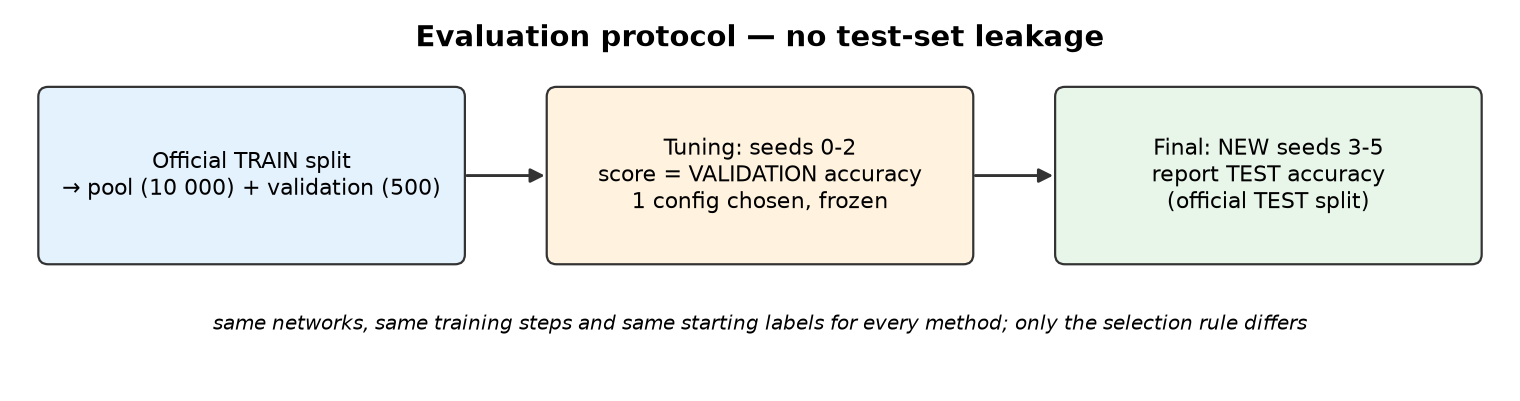
\includegraphics[width=\columnwidth]{protocol.png}
\caption{Evaluation protocol: tuning on validation data (seeds 0--2), reporting on the test split (seeds 3, 4, 5).}
\label{fig:protocol}
\end{figure}

\section{Results}
Table~\ref{tab:main} reports held-out AULC. DualNet-AL v2 is the best of nine methods on SVHN and CIFAR-10 and second on
Fashion-MNIST, where Margin is 0.17 pp higher. Table~\ref{tab:pair} compares v2 with Random on identical seeds
and starting labels: v2 is better on every seed of every dataset, by +2.41, +4.38 and +1.46 pp
AULC, and reaches Random's final (900-label) accuracy after about 346,
715 and 684 labels.

\begin{table}[t]
\caption{Held-out AULC (\%), mean $\pm$ std over seeds 3, 4, 5. Best in bold.}
\label{tab:main}
\centering\footnotesize
\resizebox{\columnwidth}{!}{%
\begin{tabular}{lccc}
\toprule
Method & Fashion-MNIST & SVHN & CIFAR-10 \\
\midrule
Random & 78.92$\pm$1.18 & 53.17$\pm$1.49 & 47.20$\pm$0.30 \\
Entropy~\cite{lewis1994} & 77.86$\pm$0.88 & 38.71$\pm$1.57 & 45.88$\pm$1.01 \\
Margin~\cite{scheffer2001} & \textbf{81.49$\pm$0.38} & 49.34$\pm$2.70 & 47.95$\pm$0.21 \\
BALD~\cite{houlsby2011,gal2017} & 79.94$\pm$0.48 & 55.89$\pm$1.25 & 47.05$\pm$1.19 \\
Core-Set~\cite{sener2018} & 78.42$\pm$0.66 & 40.18$\pm$1.65 & 46.81$\pm$1.17 \\
QBC~\cite{seung1992} & 79.63$\pm$0.81 & 47.58$\pm$1.77 & 46.30$\pm$0.64 \\
DualNet-AL v1 (fixed) & 80.72$\pm$0.82 & 51.08$\pm$1.56 & 48.46$\pm$0.34 \\
DualNet-AL v1 (meta) & 80.04$\pm$0.67 & 49.30$\pm$4.34 & 48.26$\pm$0.68 \\
\textbf{DualNet-AL v2 (ours)} & 81.33$\pm$0.34 & \textbf{57.56$\pm$1.12} & \textbf{48.66$\pm$0.52} \\
\bottomrule
\end{tabular}}
\end{table}

\begin{table*}[t]
\caption{DualNet-AL v2 vs Random on the same held-out seeds (v2 / Random).}
\label{tab:pair}
\centering\small
\begin{tabular}{lcccccc}
\toprule
Dataset & $\Delta$AULC (pp) & Seeds better & Final acc. & Macro-F1 & Worst-class recall & Labels to Random@900 \\
\midrule
Fashion-MNIST & +2.41 & 3/3 & 83.65 / 81.02 & 83.51 / 80.72 & 46.8 / 38.0 & 346 \\
SVHN & +4.38 & 3/3 & 69.70 / 70.20 & 65.77 / 63.91 & 40.5 / 16.7 & 715 \\
CIFAR-10 & +1.46 & 3/3 & 53.98 / 52.93 & 53.07 / 51.70 & 27.9 / 21.2 & 684 \\
\bottomrule
\end{tabular}
\end{table*}

Uncertainty-only methods collapse on SVHN (Entropy 38.71\%, Core-Set
40.18\% vs Random 53.17\%): with a few hundred labels their batches are dominated by
confusing, redundant digits. DualNet-AL v1 also lost to Random there (49.30\%), which
motivated v2. Worst-class recall rises from 16.7\% to 40.5\% on SVHN, from 38.0\% to 46.8\% on
Fashion-MNIST and from 21.2\% to 27.9\% on CIFAR-10 (Fig.~\ref{fig:gain}, Fig.~\ref{fig:curves}).

\begin{figure}[t]
\centering
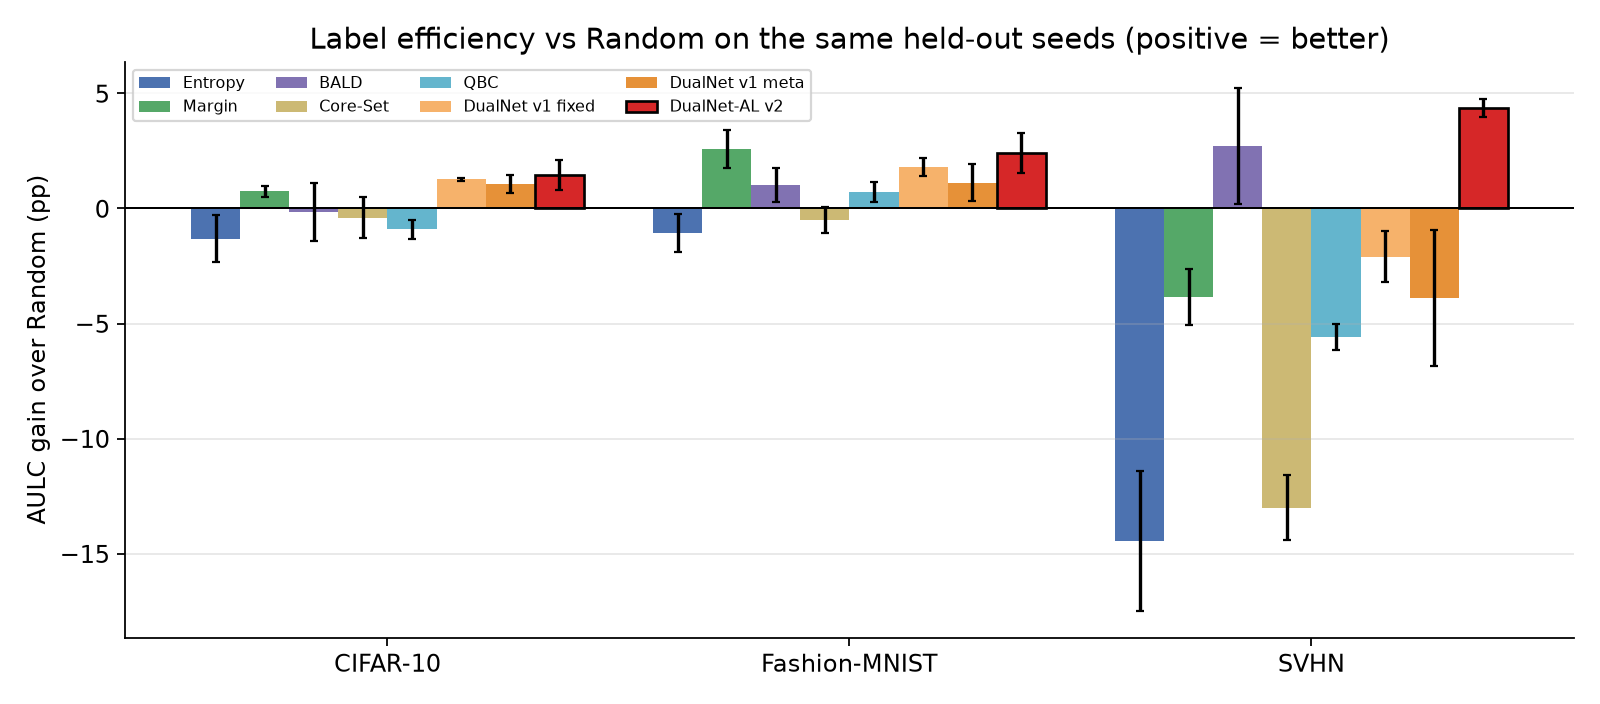
\includegraphics[width=\columnwidth]{gain_vs_random.png}
\caption{AULC gain over Random on the same held-out seeds (error bars: std over seeds).}
\label{fig:gain}
\end{figure}

\begin{figure*}[t]
\centering
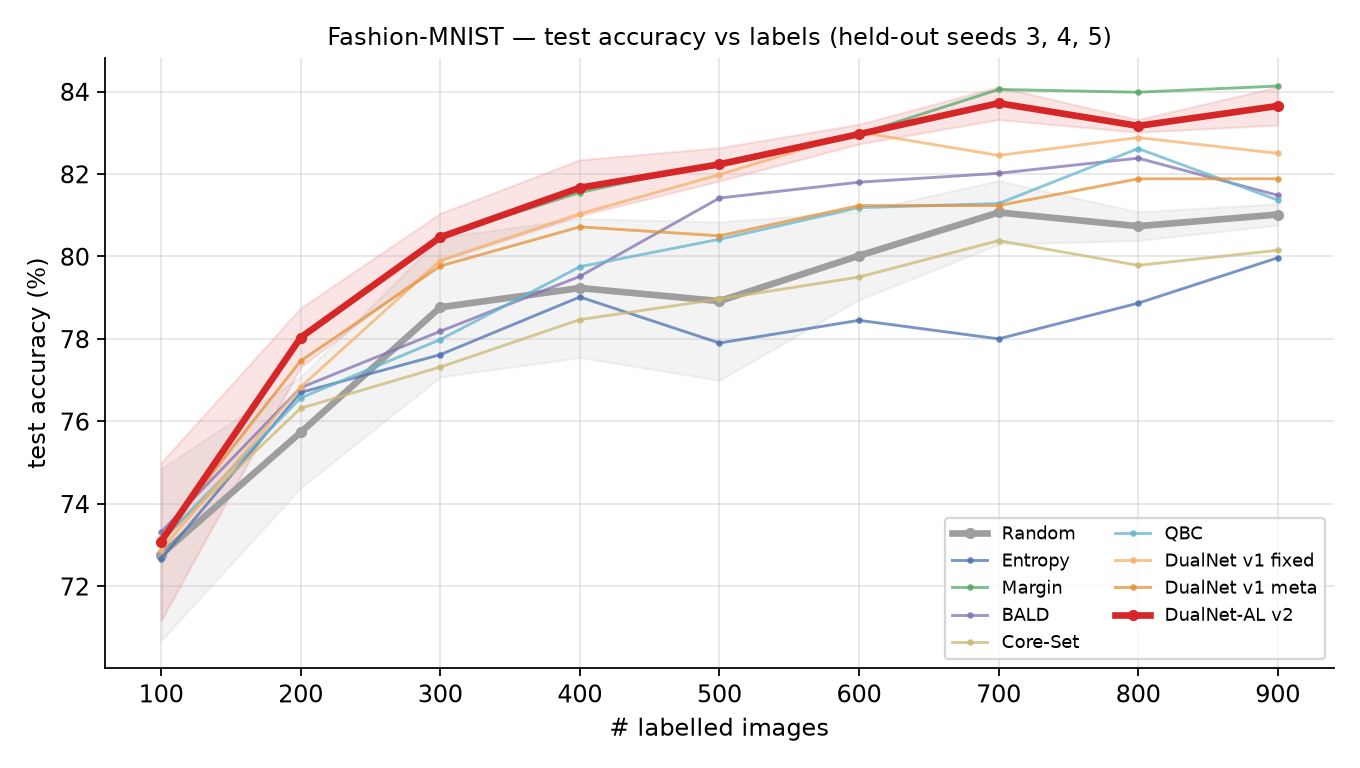
\includegraphics[width=0.32\textwidth]{curve_fmnist.png}\hfill
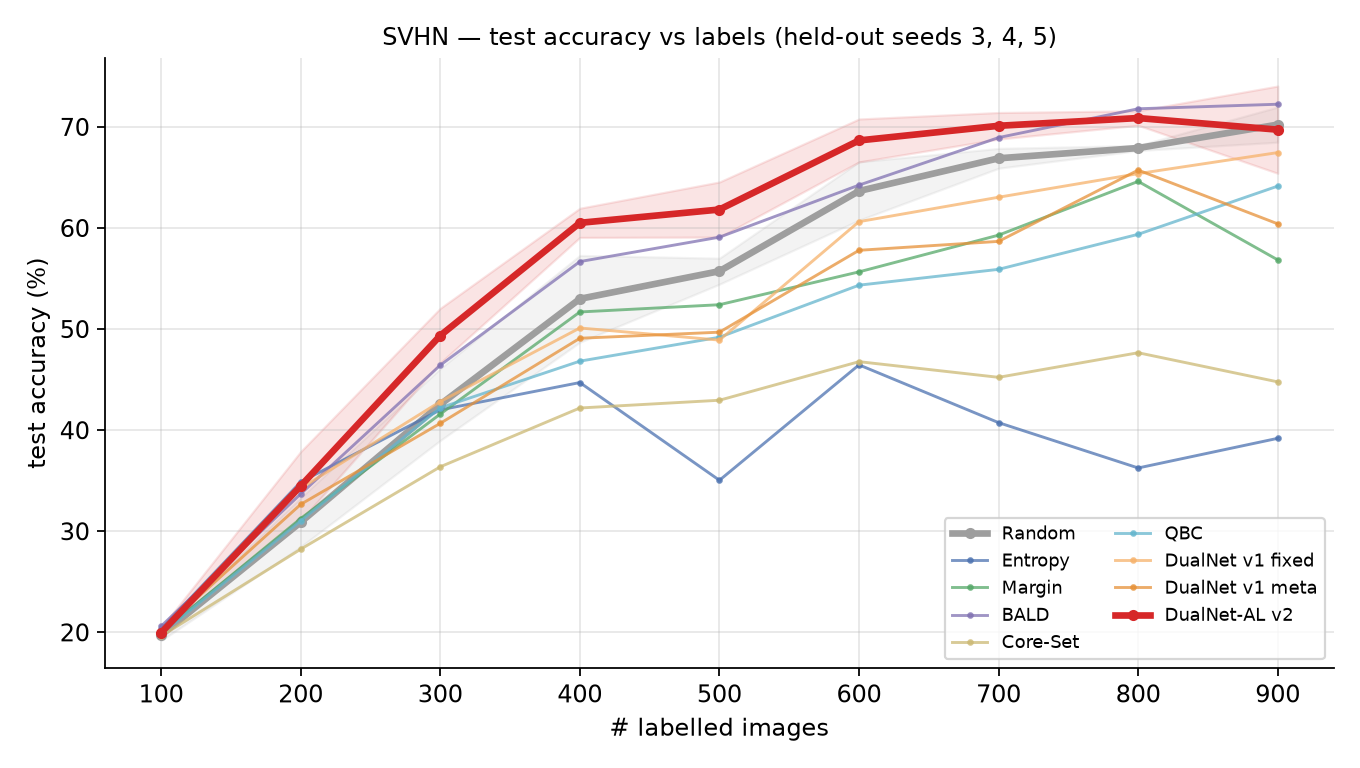
\includegraphics[width=0.32\textwidth]{curve_svhn.png}\hfill
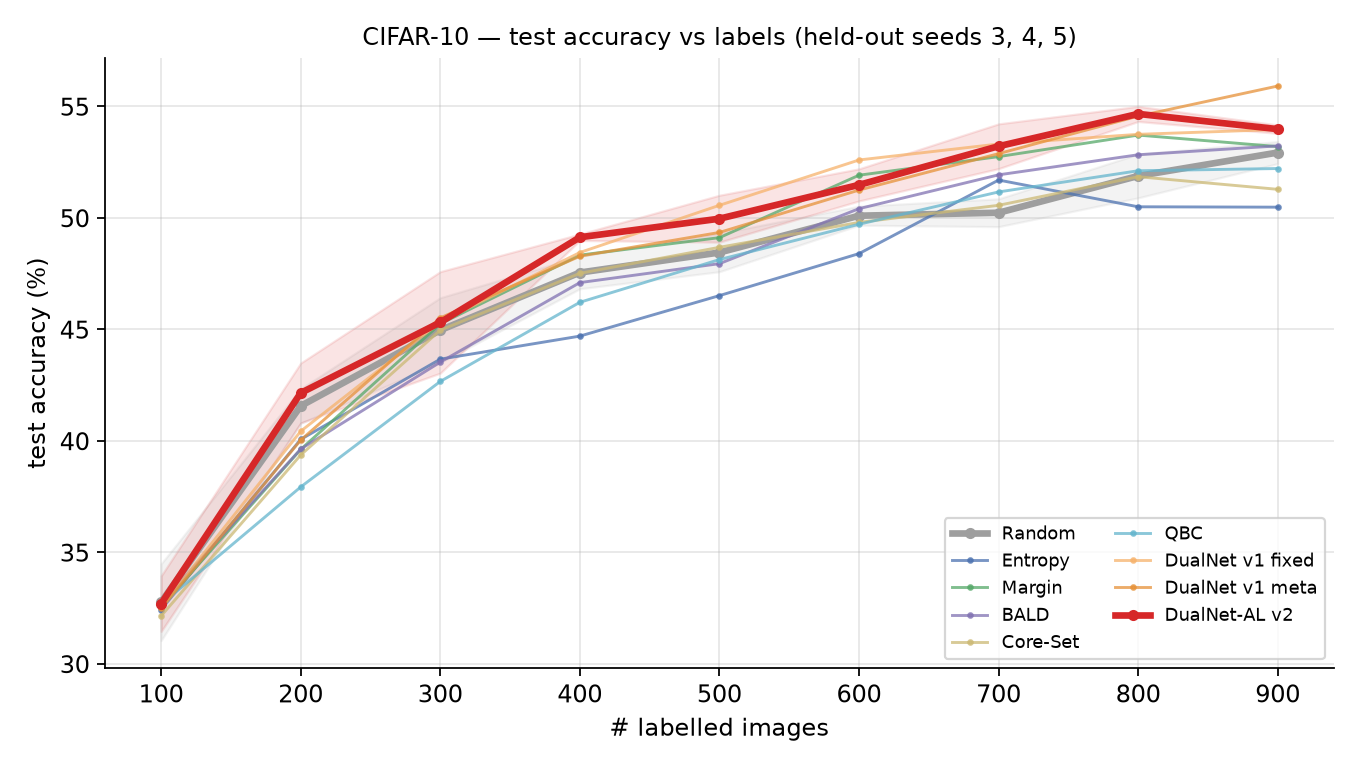
\includegraphics[width=0.32\textwidth]{curve_cifar10.png}
\caption{Test accuracy vs number of labels (mean $\pm$ std over held-out seeds). Left to right: Fashion-MNIST, SVHN,
CIFAR-10.}
\label{fig:curves}
\end{figure*}

\subsection{Ablation and tuning}
Table~\ref{tab:tune} lists the validation results used for model selection. Removing the budget-aware prior
($\lambda=1$ throughout) costs 4.93 pp on SVHN and 1.90 pp on CIFAR-10 relative to the chosen setting
(-0.08 pp on Fashion-MNIST), confirming that typical samples matter most while labels are scarce. With the same
schedule, entropy instead of margin uncertainty changes validation AULC by -0.31, -0.26 and
-0.65 pp, so margin was kept. Because the best setting differs between datasets, one configuration was chosen
by mean gain rather than tuned per dataset.

\begin{table}[t]
\caption{Validation AULC (\%) on tuning seeds 0--2 (test set unused). $\checkmark$ = chosen.}
\label{tab:tune}
\centering\footnotesize
\resizebox{\columnwidth}{!}{%
\begin{tabular}{lcccc}
\toprule
Configuration & Fashion-MNIST & SVHN & CIFAR-10 & Mean $\Delta$ \\
\midrule
$\lambda_0{=}0$, $r{=}4$, margin & 79.33 & 58.89 & 48.18 & +2.13 \\
$\lambda_0{=}0$, $r{=}8$, margin & 79.20 & 58.85 & 47.40 & +1.82 \\
$\lambda_0{=}0.5$, $r{=}4$, margin $\checkmark$ & 79.75 & 57.53 & 49.19 & +2.16 \\
$\lambda_0{=}0$, $r{=}4$, entropy & 79.03 & 58.63 & 47.53 & +1.73 \\
no prior ($\lambda{=}1$), margin & 79.83 & 52.61 & 47.29 & -0.09 \\
$\lambda_0{=}0$, $r{=}2$, margin & 79.28 & 59.04 & 48.07 & +2.13 \\
DualNet-AL v1 meta (ref.) & 79.27 & 54.23 & 47.98 & +0.49 \\
Random (ref.) & 78.46 & 53.48 & 48.05 & -- \\
\bottomrule
\end{tabular}}
\end{table}

\subsection{Cost and calibration}
Selection adds about one second per round on the GPU (Table~\ref{tab:cost}), small next to retraining two networks;
GPU $k$-means reduced v2's selection from 48\,s to 0.03\,s per round in our implementation. A weakness is calibration:
v2 has a higher ECE than Random, consistent with deliberately skewed training sets; temperature
scaling~\cite{guo2017} is a direct remedy not yet applied.

\begin{table}[t]
\caption{Mean selection time per round (s) and mean final ECE.}
\label{tab:cost}
\centering\footnotesize
\resizebox{\columnwidth}{!}{%
\begin{tabular}{lcccc}
\toprule
Method & Fashion-MNIST & SVHN & CIFAR-10 & ECE \\
\midrule
Random & 2.40 & 1.37 & 0.66 & 0.144 \\
BALD~\cite{houlsby2011,gal2017} & 3.00 & 2.14 & 0.82 & 0.187 \\
Core-Set~\cite{sener2018} & 2.57 & 1.57 & 0.79 & 0.172 \\
DualNet-AL v1 (meta) & 2.85 & 2.22 & 1.08 & 0.227 \\
\textbf{DualNet-AL v2 (ours)} & 0.98 & 1.11 & 1.12 & 0.217 \\
\bottomrule
\end{tabular}}
\end{table}

\section{Discussion and Limitations}
The results support the hypothesis that no single criterion suits every dataset and budget, and that scheduling from
typicality to learned informativeness, with cluster-level diversity, is more robust than a fixed rule. Budgets are
small ($\le$900 labels) and pools are 10\,000 images, so absolute accuracies are below full-data numbers and gaps are
a few points. Three held-out seeds give a consistent paired comparison but not a formal significance test. On SVHN,
v2's final accuracy (69.70\%) is slightly below Random's (70.20\%) although it is
ahead for almost the whole curve. The meta-learner's reward uses a 500-image validation set that the baselines do not
use. BADGE~\cite{ash2020}, learning loss~\cite{yoo2019}, CIFAR-100 and long-tailed data are not yet evaluated.

\section{Conclusion}
DualNet-AL combines two complementary networks, five acquisition signals with meta-learned weights, a budget-aware
typicality prior and cluster-based batches. Under a leak-free protocol it beats random sampling on all three datasets
and all held-out seeds, and is the best of nine methods on two of them. Future work covers larger budgets, more seeds
with significance testing, a label-free meta reward, calibration, stronger backbones and further baselines.

\section*{Code availability}
Code, per-run logs, the chosen configuration and a one-command demo: \url{https://github.com/iamthehimansh/DualNet-AL_Motion}.

\begin{thebibliography}{99}
\bibitem{settles2009} B.~Settles, ``Active learning literature survey,'' Computer Sciences Technical Report 1648, University of Wisconsin--Madison, 2009.
\bibitem{lewis1994} D.~D. Lewis and W.~A. Gale, ``A sequential algorithm for training text classifiers,'' in \emph{Proc. ACM SIGIR}, 1994, pp. 3--12.
\bibitem{scheffer2001} T.~Scheffer, C.~Decomain, and S.~Wrobel, ``Active hidden {M}arkov models for information extraction,'' in \emph{Proc. Int. Symp. Intelligent Data Analysis}, 2001, pp. 309--318.
\bibitem{seung1992} H.~S. Seung, M.~Opper, and H.~Sompolinsky, ``Query by committee,'' in \emph{Proc. 5th Annual Workshop on Computational Learning Theory}, 1992, pp. 287--294.
\bibitem{houlsby2011} N.~Houlsby, F.~Husz\'ar, Z.~Ghahramani, and M.~Lengyel, ``Bayesian active learning for classification and preference learning,'' arXiv:1112.5745, 2011.
\bibitem{gal2017} Y.~Gal, R.~Islam, and Z.~Ghahramani, ``Deep {B}ayesian active learning with image data,'' in \emph{Proc. ICML}, 2017.
\bibitem{sener2018} O.~Sener and S.~Savarese, ``Active learning for convolutional neural networks: A core-set approach,'' in \emph{Proc. ICLR}, 2018.
\bibitem{ash2020} J.~T. Ash, C.~Zhang, A.~Krishnamurthy, J.~Langford, and A.~Agarwal, ``Deep batch active learning by diverse, uncertain gradient lower bounds,'' in \emph{Proc. ICLR}, 2020.
\bibitem{yoo2019} D.~Yoo and I.~S. Kweon, ``Learning loss for active learning,'' in \emph{Proc. IEEE/CVF CVPR}, 2019.
\bibitem{hacohen2022} G.~Hacohen, A.~Dekel, and D.~Weinshall, ``Active learning on a budget: Opposite strategies suit high and low budgets,'' in \emph{Proc. ICML}, 2022.
\bibitem{konyushkova2017} K.~Konyushkova, R.~Sznitman, and P.~Fua, ``Learning active learning from data,'' in \emph{Proc. NeurIPS}, 2017.
\bibitem{hsu2015} W.-N. Hsu and H.-T. Lin, ``Active learning by learning,'' in \emph{Proc. AAAI}, 2015.
\bibitem{nguyen2004} H.~T. Nguyen and A.~Smeulders, ``Active learning using pre-clustering,'' in \emph{Proc. ICML}, 2004.
\bibitem{lin1991} J.~Lin, ``Divergence measures based on the {S}hannon entropy,'' \emph{IEEE Trans. Inf. Theory}, vol.~37, no.~1, pp. 145--151, 1991.
\bibitem{williams1992} R.~J. Williams, ``Simple statistical gradient-following algorithms for connectionist reinforcement learning,'' \emph{Machine Learning}, vol.~8, pp. 229--256, 1992.
\bibitem{arthur2007} D.~Arthur and S.~Vassilvitskii, ``k-means++: The advantages of careful seeding,'' in \emph{Proc. ACM-SIAM SODA}, 2007.
\bibitem{xiao2017} H.~Xiao, K.~Rasul, and R.~Vollgraf, ``Fashion-{MNIST}: A novel image dataset for benchmarking machine learning algorithms,'' arXiv:1708.07747, 2017.
\bibitem{krizhevsky2009} A.~Krizhevsky, ``Learning multiple layers of features from tiny images,'' Technical Report, University of Toronto, 2009.
\bibitem{netzer2011} Y.~Netzer, T.~Wang, A.~Coates, A.~Bissacco, B.~Wu, and A.~Y. Ng, ``Reading digits in natural images with unsupervised feature learning,'' in \emph{NIPS Workshop on Deep Learning and Unsupervised Feature Learning}, 2011.
\bibitem{guo2017} C.~Guo, G.~Pleiss, Y.~Sun, and K.~Q. Weinberger, ``On calibration of modern neural networks,'' in \emph{Proc. ICML}, 2017.
\bibitem{paszke2019} A.~Paszke \emph{et~al.}, ``{PyTorch}: An imperative style, high-performance deep learning library,'' in \emph{Proc. NeurIPS}, 2019.
\bibitem{blum1998} A.~Blum and T.~Mitchell, ``Combining labeled and unlabeled data with co-training,'' in \emph{Proc. COLT}, 1998.
\end{thebibliography}
\end{document}
